\documentclass{article}
\usepackage[in]{fullpage}
\usepackage{tikz}
\usepackage{amsmath}
\usepackage{amsfonts}
\usepackage{bm}
%
\begin{document}
%\pdfpageheight=10in
%\pdfpagewidth=9in
%
% paper title
\title{ANN}
%\author{Craig~Euler}
%
\maketitle
Unfinished, generic network-topology figure:
%
\begin{center}
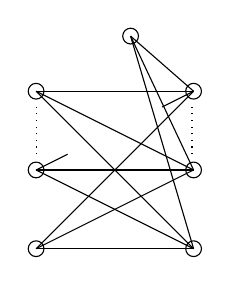
\begin{tikzpicture}
\draw (0.0, 0.0) circle (0.1cm);
\draw (0.0, 1.0) circle (0.1cm);
\draw (0.0, 2.0) circle (0.1cm);

\draw (2.0, 2.0) circle (0.1cm);
\draw (2.0, 0.0) circle (0.1cm);
\draw (2.0, 1.0) circle (0.1cm);
\draw (1.2, 2.7) circle (0.1cm);

\draw (0.0, 0.0) -- (2.0, 0.0);
\draw (0.0, 0.0) -- (2.0, 1.0);
\draw (0.0, 0.0) -- (2.0, 2.0);

\draw (0.0, 1.0) -- (2.0, 0.0);
\draw (0.0, 1.0) -- (2.0, 1.0);
\draw (0.0, 1.0) -- (0.4, 1.2);
\draw (1.6, 1.8) -- (2.0, 2.0);

\draw (0.0, 2.0) -- (2.0, 0.0);
\draw (0.0, 2.0) -- (2.0, 1.0);
\draw (0.0, 2.0) -- (2.0, 2.0);

\draw (1.2, 2.7) -- (2.0, 0.0);
\draw (1.2, 2.7) -- (2.0, 1.0);
\draw (1.2, 2.7) -- (2.0, 2.0);
\draw[dotted] (0.01, 1.2) -- (0.01, 1.8);
\draw[dotted] (1.98, 1.2) -- (1.98, 1.8);
\end{tikzpicture}
\end{center}
%
Back propagation derivation for the traditional ANN.

A caveat: the range for summation indexing is assumed from its context in these notes.
Since no absolute frame of reference will be necessary, a term such as $k \in M$ will refer to indexing over $M \subset \mathbb{Z}$ and $N$ will refer to the number of layers in the network.

First define some shorthand $\psi_p^q$ to be the $p^{th}$ element of the result of the corresponding weights applied to the nodes at the $q^{th}$ layer along with the bias term $b^q$ (often just 1) and bias weight $u_p^q$:
%
\begin{equation} \label{eq:psi}
\psi_p^q = \sum_{k \in M^q} y_k^q \omega_{p,k}^q + b^q u_p^q, \; \; \; \; \; \forall p \in M^{q+1}.
\end{equation}
%
For reference, it follows that
%
\begin{equation} \label{eq:dpsi_w}
\frac{\partial \psi_p^q}{\partial \omega_{s,r}^q} =
\begin{cases}
y_r^q, & p = s \\
0, & p \neq s
\end{cases}
\end{equation}
%
\begin{equation} \label{eq:dpsi_u}
\frac{\partial \psi_p^q}{\partial u_p^q} =
b^q
\end{equation}
%
and
%
\begin{equation} \label{eq:dpsi_y}
\frac{\partial \psi_p^q}{\partial y_r^q} =
\omega_{p,r}^q
\end{equation}
%
%\begin{equation} \label{eq:dpsi_w}
%\frac{\partial \psi_p^q}{\partial \omega_{q,r}^q} =
%\begin{cases}
%\sum_{k \in M^q} y_k^q \omega_{p,k}^q + b^iu_p^q, & 1 \\
%k, & 2
%\end{cases}
%\end{equation}
%
Superscripts refer to the specified layer.
Hence, \eqref{eq:psi} will refer to the $q^{th}$ layer before undergoing activation.
%
where $g$ is the activation function. The sigmoid function is defined as:
%
\begin{equation} \label{eq:g}
g(x;\beta) := \frac{1}{1 + e^{-\beta x}}
\end{equation}
%
which is the activation function of choice here.
It follows that
%
\begin{equation} \label{eq:gp}
\frac{d g}{d x} = \beta \left( 1 - g(x;\beta) \right) g(x; \beta).
\end{equation}
%
To keep the activation function generic, $g'$ will be used to refer to its derivative.

Promotion to the next layer (at $q+1$) will be defined to be after the activation is performed at the current layer (at $q$):
%
\begin{equation} \label{eq:z}
y_p^{q+1} := g(\psi_p^q)
\end{equation}
%
The zero-based index is used to refer to the specified layer.
For convenience (and slight redundancy with the terms $y^0$ and $y^{N-1}$), the first, interior, and last layers are denoted with $x$, $y$, and $z$ respectively.
It follows that $x = y^0$ and $z = y^{N-1}$.
Therefore, the last layer is then:
%
\begin{equation} \label{eq:z}
z_p = g(\psi_p^{N-2})
\end{equation}
%
with $N$ denoting the number of layers of the network.
%
Let the error be defined as:
%
\begin{equation} \label{eq:error}
E := \frac{1}{2} \sum_k (z_k - t_k)^2
\end{equation}
%
then
%
\begin{equation} \label{eq:derror}
\frac{\partial E}{\partial z_p} = z_p - t_p
\end{equation}
%
\begin{equation} \label{eq:gamma}
\gamma_i := (z_i - t_i) g'(\psi_i^{N-2})
\end{equation}
%
the rate of change of the error term with the weights to the last layer is
%
\begin{equation} \label{eq:last_layer_derror}
\begin{aligned}
\frac{\partial E}{\partial \omega_{i,j}^{N-2}} &=
\left( \frac{\partial E}{\partial z_i} \right)
\left( \frac{\partial z_i}{\partial g} \right)
\left( \frac{\partial g}{\partial \psi_i^{N-2}} \right)
\left( \frac{\partial \psi_i^{N-2}}{\partial \omega_{i, j}^{N-2}} \right) \\
&=
\left( z_i - t_i \right)
\left( 1 \right)
\left( g' (\psi_i^{N-2}) \right)
\left( y_j^{N-2} \right) \\
&=
y_j^{N-2}
\left( z_i - t_i \right)
g' (\psi_i^{N-2}) \\
&=
y_j^{N-2}
\gamma_i.
\end{aligned}
\end{equation}
%
notice that
%
\begin{equation} \label{eq:last_layer_derror_eq_0}
\frac{\partial z_i}{\partial \omega_{p,j}} = 0, \ \ \ \forall i \neq p
\end{equation}
%
Likewise, the partial of the error term with the bias is:
%
\begin{equation} \label{eq:d_bias}
\frac{\partial E}{\partial u_{i}^{N-2}} =
b^{N-2}
\gamma_i.
\end{equation}
%
Expanding the derivative of the error term w.r.t. the $N-3$ layer weights:
%
\begin{equation} \label{eq:derive_du_nm3}
\begin{aligned}
\frac{\partial E}{\partial \omega_{i,j}^{N-3}} &= 
%
\sum_{k_{N-1}}
\frac{\partial E}{\partial z_{k_{N-1}}}
\frac{\partial z_{k_{N-1}}}{\partial g}
\frac{\partial g}{\partial \psi_{k_{N-1}}^{N-2}}
%
\sum_{k_{N-2}}
\frac{\partial \psi_{k_{N-1}}^{N-2}}{\partial y_{k_{N-2}}^{N-2}}
\frac{\partial y_{k_{N-2}}^{N-2}}{\partial g}
\frac{\partial g}{\partial \psi_{k_{N-2}}^{N-3}}
%
\sum_{k_{N-3}=i}
\frac{\partial \psi_{k_{N-2}}^{N-3}}{\partial \omega_{k_{N-3,j}}^{N-3}} \\
%%
& = \sum_{k_{N-1}}
\left( z_{k_{N-1}} - t_{k_{N-1}} \right)
%
(1)
\left( g' \left( \psi_{k_{N-1}}^{N-2} \right) \right)
%
\left( \omega_{k_{N-1},i}^{N-2} \right)
(1)
\left( g' (\psi_i^{N-3}) \right)
\left( y_j^{N-3} \right) \\
%%
& =
\sum_{k_{N-1}}
\left( z_{k_{N-1}} - t_{k_{N-1}} \right)
%
g' \left(\psi_{k_{N-1}}^{N-2}\right)
%
\omega_{k_{N-1},i}^{N-2}
g' \left( \psi_i^{N-3} \right)
y_j^{N-3} \\
%%
& =
\left(
\sum_{k_{N-1}}
\gamma_{k_{N-1}}
\omega_{k_{N-1},i}^{N-2}
\right)
g' \left( \psi_i^{N-3} \right)
y_j^{N-3} \\
%%
\end{aligned}
\end{equation}
%
Expanding the derivative of the error term w.r.t. the $N-4$ layer weights:
%
\begin{equation} \label{eq:derive_du_nm4}
\begin{aligned}
\frac{\partial E}{\partial \omega_{i,j}^{N-4}} =& \;
%
\sum_{k_{N-1}}
\frac{\partial E}{\partial z_{k_{N-1}}}
\frac{\partial z_{k_{N-1}}}{\partial g}
\frac{\partial g}{\partial \psi_{k_{N-1}}^{N-2}}
%
\sum_{k_{N-2}}
\frac{\partial \psi_{k_{N-1}}^{N-2}}{\partial y_{k_{N-2}}^{N-2}}
\frac{\partial y_{k_{N-2}}^{N-2}}{\partial g}
\frac{\partial g}{\partial \psi_{k_{N-2}}^{N-3}} \\
%
& \;\sum_{k_{N-3}}
\frac{\partial \psi_{k_{N-2}}^{N-3}}{\partial y_{k_{N-3}}^{N-3}}
\frac{\partial y_{k_{N-3}}^{N-3}}{\partial g}
\frac{\partial g}{\partial \psi_{k_{N-3}}^{N-4}}
%
\sum_{k_{N-4}=i}
\frac{\partial \psi_{k_{N-3}}^{N-4}}{\partial \omega_{k_{N-4,j}}^{N-4}} \\
%%
=& \; \sum_{k_{N-1}}
\left( z_{k_{N-1}} - t_{k_{N-1}} \right)
%
(1)
\left( g' \left( \psi_{k_{N-1}}^{N-2} \right) \right)
%
\sum_{k_{N-2}}
\left( \omega_{k_{N-1},k_{N-2}}^{N-2} \right)
(1)
\left( g' (\psi_{k_{N-2}}^{N-3}) \right) \\
%
& \; \left( \omega_{k_{N-2},i}^{N-3} \right)
(1)
\left( g' (\psi_i^{N-4}) \right)
%
\left( y_j^{N-4} \right) \\
%%
=& \;
\sum_{k_{N-1}}
\left( z_{k_{N-1}} - t_{k_{N-1}} \right)
g' \left( \psi_{k_{N-1}}^{N-2} \right)
%
\sum_{k_{N-2}}
\omega_{k_{N-1},k_{N-2}}^{N-2}
g' \left( \psi_{k_{N-2}}^{N-3} \right) \\
%
& \; \omega_{k_{N-2},i}^{N-3}
g' \left( \psi_i^{N-4} \right)
y_j^{N-4} \\
%%
=& \;
\left(
\sum_{k_{N-1}}
\gamma_{k_{N-1}}
%
\sum_{k_{N-2}}
\omega_{k_{N-1},k_{N-2}}^{N-2}
g' \left( \psi_{k_{N-2}}^{N-3} \right)
%
\omega_{k_{N-2},i}^{N-3} \;
\right)
g' \left( \psi_i^{N-4} \right)
y_j^{N-4} \\
%%
\end{aligned}
\end{equation}
%
\begin{equation} \label{eq:derive_du_nm5}
\frac{\partial E}{\partial \omega_{i,j}^{N-5}} =
\left(
\sum_{k_{N-1}}
\gamma_{k_{N-1}}
%
\sum_{k_{N-2}}
\omega_{k_{N-1},k_{N-2}}^{N-2}
g' \left( \psi_{k_{N-2}}^{N-3} \right)
%
\sum_{k_{N-3}}
\omega_{k_{N-2},k_{N-3}}^{N-3}
g' \left( \psi_{k_{N-3}}^{N-4} \right)
%
\omega_{k_{N-3},i}^{N-4} \;
\right)
g' \left( \psi_i^{N-5} \right)
y_j^{N-5} \\
%
\end{equation}
%
letting $\bm{\gamma}$ and $\bm{y}$ be row vectors and the $\bm{\psi}$ terms be column vectors, \eqref{eq:derive_du_nm5} can then be expressed as:
%
\begin{equation} \label{eq:derive_du_nm5_matrix}
\frac{\partial \bm{E}}{\partial \bm{\omega}^{N-5}} =
\left(
\left(
\bm{\gamma} \;
\bm{\omega}^{N-2} \;
g' (\bm{\psi}^{N-3}) \;
\bm{\omega}^{N-3} \;
g' (\bm{\psi}^{N-4}) \;
\bm{\omega}^{N-4} \;
\right)^T \;
\cdots
\right) \;
\odot
\left(
g' (\bm{\psi}^{N-5})
\bm{y}^{N-5} \\
\right)
\end{equation}
%
where $\cdots$ represents the terms repeated to the appropriate size to perform the Hadamard product.
More generally, using the following definition:
%
\begin{equation} \label{eq:delta}
\bm{\delta}^q := \bm{\omega}^q \; g' \left( \bm{\psi}^{q-1} \right)
\end{equation}
%
\begin{equation} \label{eq:derive_du_nm5_matrix_delta}
\frac{\partial \bm{E}}{\partial \bm{\omega}^{N-p}} =
\left(
\left(
\bm{\gamma} \;
\prod_{q=2}^{p-3}
\left( \bm{\omega}^{N-q} * g' \left( \bm{\psi}^{N-q-1} \right) \right)
\bm{\omega}^{N-(p-1)}
\right)^T
\cdots
\right) \;
\odot
\left(
g' \left( \bm{\psi}^{N-p} \right)
\bm{y}^{N-p}
\right)
\end{equation}
%
Choosing a step size $\eta > 0$, gradient descent is applied at each layer, $q \in [0, N-1)$, to advance the network weights to the next iteration as follows:
%
\begin{equation} \label{eq:end_weights}
\omega_{new}^q = \omega_{old}^q - \eta
\frac{\partial \bm{E}}{\partial \bm{\omega}^q}
\end{equation}
%
\end{document}
